\documentclass{article}

\newcommand{\authorname}{Austin Jetrin Maddison}
\newcommand{\course}{Discrete Simulation}
\newcommand{\courseid}{ICMA393}
\newcommand{\docname}{HW3}
\newcommand{\titletext}{\course: \docname}

%\usepackage{fontspec}	
\usepackage[no-math]{fontspec}	
\setmainfont{HelveticaNowText}
\newfontface\hh{HelveticaNowText-ExtraBold}
\newfontface\lt{HelveticaNowText-Light}      
\newfontface\xx{HelveticaNowText-ExtraLight} 
\newfontface\mm{HelveticaNowText Medium}

\newfontfamily{\displayfont}{HelveticaNowDisplay}
\newfontface\dslt{HelveticaNowDisplay-Light}
\newfontface\dsmm{HelveticaNowDisplay-Medium}
\newfontface\dsbd{HelveticaNowDisplay-Bold}

\newfontfamily{\microfont}{HelveticaNowMicro}
\newfontface\mclt{HelveticaNowMicro-Light}
\newfontface\mcmm{HelveticaNowMicro-Medium}
\newfontface\mcbd{HelveticaNowMicro-Bold}

\setmonofont{SFMono}

\usepackage[lining]{FiraSans}
\usepackage[fakebold]{firamath-otf}
\usepackage{unicode-math}
\setmathfont{FiraMath}
\renewcommand*\oldstylenums[1]{{\firaoldstyle #1}}


\usepackage{microtype}   % Improves text appearance with microtypography
\usepackage{amsmath}     % For better math support
\usepackage{graphicx}    % For including graphics
\usepackage{lipsum}      % For placeholder text
\usepackage{enumitem}
\usepackage{xcolor}
\usepackage{svg}
\usepackage{svg-extract}
\usepackage{caption}
\usepackage{float}
\usepackage{multicol}
\usepackage{booktabs}



\usepackage[a4paper, margin=0.8in, columnsep=20pt]{geometry}

\captionsetup{font=small}
\definecolor{gray}{rgb}{0.55, 0.55, 0.55}
\setlength{\columnsep}{20pt}  % Space between columns

% Headers and Footers
\usepackage{fancyhdr}
\pagestyle{fancy}
\fancyhf{}

% First Page
\fancypagestyle{plain}{
\fancyfoot[R]{\small \thepage} 
\fancyfoot[L]{} 
\fancyhead[L]{}
\fancyhead[R]{}
}

% Custom header
\fancyfoot[L]{\scriptsize \MakeUppercase{ \microfont \courseid~\course}}
\fancyhead[L]{\scriptsize \MakeUppercase{ \microfont \docname}}
\renewcommand{\headrulewidth}{0pt}

% Custom footer
%\fancyfoot[L]{\small Title, Date}
\fancyfoot[R]{\small \thepage}

% Line spacing
\usepackage{setspace}
\setstretch{1.15}  % Slightly more space between lines

%\setlength{\mathindent}{0pt} % This removes the indentation for equations

% Section formatting
\usepackage{titlesec}
\titleformat{\section}[block]{\large\dsbd}{\thesection.}{1em}{}
\titleformat{\subsection}[block]{\normalsize \mm}{\thesubsection.}{1em}{}

% Bibliography style
\usepackage[numbers,sort&compress]{natbib} % For numbered citations

% Hyperlinks
\usepackage{hyperref}
\hypersetup{
    colorlinks=false,
    linkcolor=blue,
    citecolor=blue,
    urlcolor=blue,
    pdftitle={Research Paper Title},
    pdfauthor={Author's Name},
}

\usepackage{listings}
\lstset{
  language=Python,                     % Use Python language syntax
  basicstyle=\ttfamily\footnotesize,           % Use modern monospace font for code
  keywordstyle=\bfseries\color{black},   % Bold and blue keywords
  stringstyle=\color{black},              % Strings in red
  commentstyle=\color{gray},            % Comments in gray
  showstringspaces=false,               % Don't show spaces in strings
  breaklines=true,                      % Break long lines
  tabsize=4,                            % Set tab size to 4 spaces
}


\begin{document}
\fontsize{9.5}{11.5}\selectfont % Set font size to 12pt with a baseline of 14pt

% Title 
\title{
  \raggedright
  \Large \displayfont \strong{\courseid~\titletext} \\[5pt]  % Adjust spacing if needed
%  \raggedleft
  \small Mahidol University International College \\
  \small \authorname \\ 
  \small \today
}
\date{} 

%
%\twocolumn[{
%	\vspace*{-1cm}
%	\maketitle
%	\vspace*{-0.5cm}
%}]

\maketitle
%\raggedbottom
\section*{Problem 1}

\noindent
I ran the simulation for N=100000 iterations, for the $U(0,U(0,U(0,U(0,371))))$.

\begin{multicols}{2}
\begin{lstlisting}
def chain_dist(chains=4, L=0, U=371):
	if chains == 0:
		return np.random.randint(L, U) 
	
	U_new = chain_dist(chains-1, L, U)
	if U_new == L : return U_new
	
	return np.random.randint(L, U_new)
	
f = np.vectorize(lambda x : chain_dist())
leading_digit =  np.vectorize(lambda _: int(str(np.abs(_))[0]))

N = 1000000
res = leading_digit( f( np.zeros(N) ) )
\end{lstlisting}
	
	
\columnbreak

\begin{figure}[H]
	\centering
	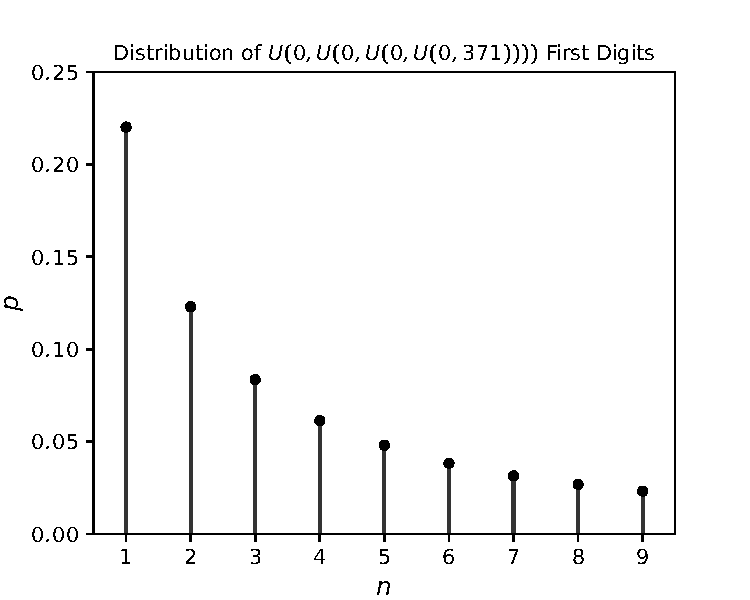
\includegraphics[width=1\linewidth]{../drawings/p1}
	%	\caption{}
	%	\label{fig:path1}
\end{figure}


\end{multicols}


\section*{Problem 2}


%\begin{multicols}{2}
	

\begin{lstlisting}
df = pd.read_csv('../data/stars.csv')
# ['Temperature (K)', 'Luminosity(L/Lo)', 'Radius(R/Ro)','Absolute magnitude(Mv)']

for i, col in enumerate(cols):
	res = leading_digit(df[col].values)
	plot(res)

\end{lstlisting}
	
		
\begin{figure}[H]
	\centering
	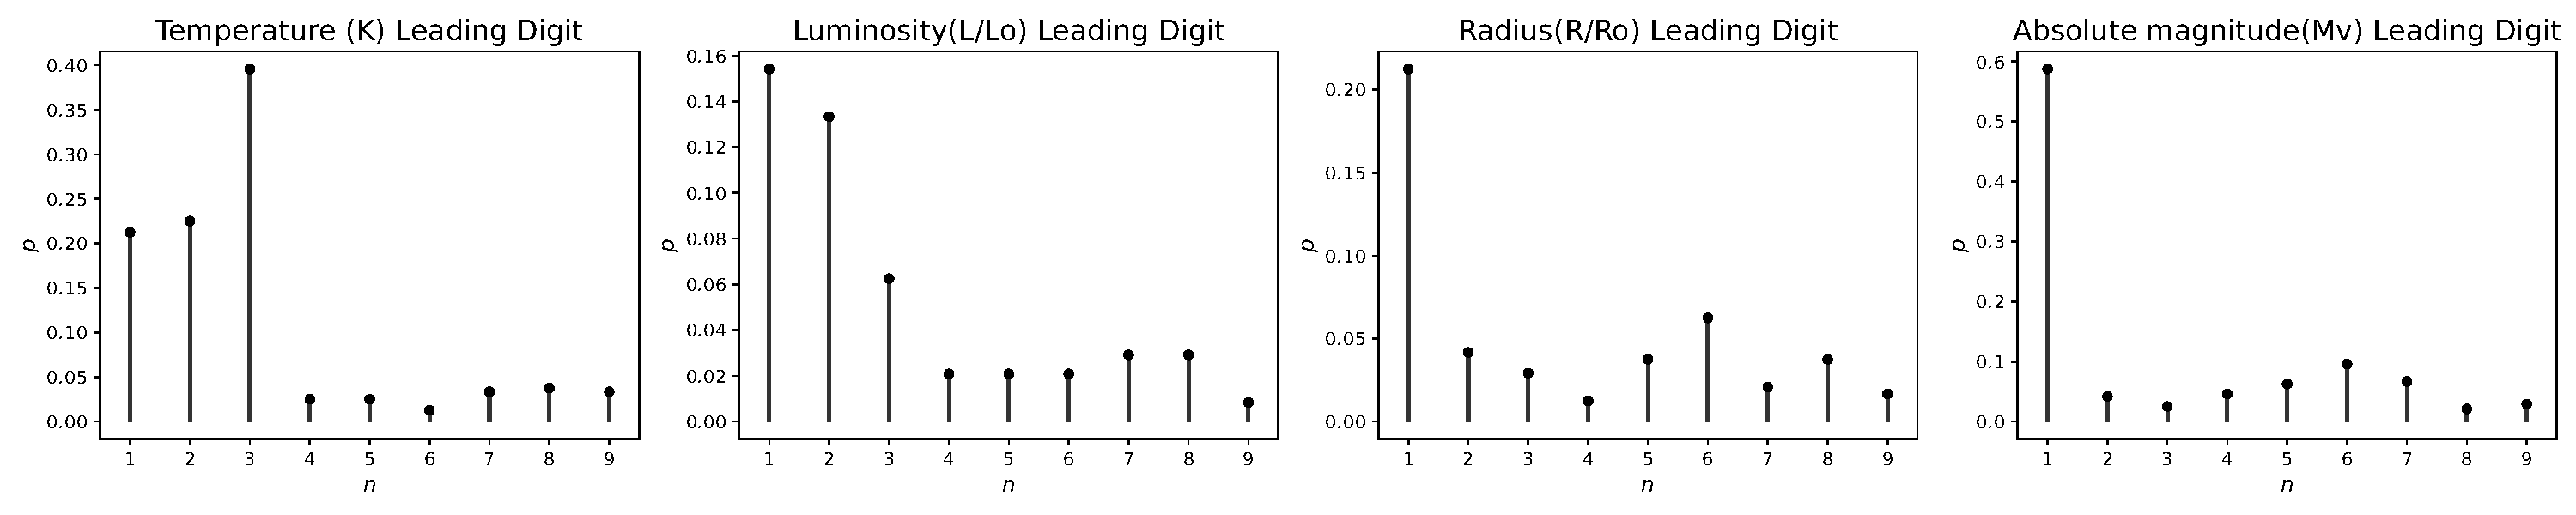
\includegraphics[width=1\linewidth]{../drawings/p2_subplots.pdf}
	%	\caption{}
	%	\label{fig:path1}
\end{figure}

%\end{multicols}

\pagebreak
\section*{Problem 3}

\begin{multicols}{2}


\begin{lstlisting}
# (a)
C.guess([0, 1, 1, 4, 9, 25, 64, 169, 441, 1156]) 
\end{lstlisting}
ans = $\frac{(-x^2 + x)}{(x^3 - 2*x^2 - 2*x + 1)}$


\begin{lstlisting}
# (b)
C.guess([i**2 for i in range(10)]) 
\end{lstlisting}
ans = $\frac{(-x^2 - x)}{(x^3 - 3*x^2 + 3*x - 1)}$
\\
\columnbreak

\begin{lstlisting}
# (c)
C.guess([int((i/2)**3)//1 for i in range(30)]) 
\end{lstlisting}
ans = $\frac{(x^10 - 2*x^9 + 4*x^8 - 2*x^7 + 3*x^6 - x^5 + 2*x^4 + x^2)}{(x^11 - 3*x^10 + 3*x^9 - x^8 - x^3 + 3*x^2 - 3*x + 1)}$

\noindent


\end{multicols}

\section*{Problem 4}
Guess the C-finite relation of the number of palindromic compositions of n.
\vspace{10pt}


\begin{lstlisting}
def find_all_sums(target_sum):
	def find_sums_recursive(remaining_sum, possible_numbers, current_combination, all_combinations):
		if remaining_sum == 0:
		all_combinations.append(current_combination)
		return
		for x in possible_numbers:
		if x <= remaining_sum:
		find_sums_recursive(remaining_sum - x, possible_numbers, current_combination + [x], all_combinations)

	possible_numbers = [num for num in range(1, target_sum + 1)]
	all_combinations = []
	find_sums_recursive(target_sum, possible_numbers, [], all_combinations)
	return all_combinations

def is_palindromic(sequence):
	if len(sequence) < 2:
		return True
	return sequence == sequence[::-1]

def find_all_palindromic_sums(target_sum):
	return [s for s in find_all_sums(target_sum) if is_palindromic(s)]

calc_length_of_palindromic_sums = lambda x : len(find_all_palindromic_sums(x))
guess_c_finite([ calc_length_of_palindromic_sums(i) for i in range(1, 20)])
\end{lstlisting}

\noindent
ans = $c_0 = 0, c_1 = -2 $

\pagebreak

\section*{Problem 5}
a) Find a formula for $a_n$
\begin{lstlisting}
	c1 = symbols('c1')
	c2 = symbols('c2')
	c3 = symbols('c3')
	c4 = symbols('c4')
	c5 = symbols('c5')
	c6 = symbols('c6')
	
	eqs = []
	for i in range(0,6):
		eqs += [(Eq(2 ** i * (c1 + i*c2 + i**2* c3 + i**3 * c4) + 3 ** i * (c5 + c6*i), given_cfinite_seq(i)))]
	sol = solve(eqs, (c1, c2, c3, c4, c5, c6))
	# sol = {c1: -1, c2: 0, c3: -9, c4: 0, c5: 1, c6: 1}
	
	print(f"= 2^n({sol[c1]} + n*{sol[c2]} + n^2* {sol[c3]} + n^3 * {sol[c4]}) + 3^n * ({sol[c5]} + {sol[c6]}*n)")
	
\end{lstlisting}
ans = $2^n(-1 + 0*n + n^2 * -9 + n^3 * 0) + 3^n * (1 + 1*n)$
\vspace{20pt}

\noindent
b)
Is there a linear recurrence for the same sequence 	for a smaller value of d? If not, explain why.

\begin{lstlisting}
	seq d=5 guess_c_finite() =  {c0: -12, c1: 57, c2: -134, c3: 156, c4: -72}
	seq d=6 guess_c_finite() =  {c0: -12, c1: 57, c2: -134, c3: 156, c4: -72}
\end{lstlisting}

\begin{table}[ht]
	\centering
 	\small % Change text size to small
    \begin{tabular}{rrr}
		\toprule
		\textbf{Index} & \textbf{seq d=5} & \textbf{seq d=6} \\
		\midrule
        0 & 0 & 0 \\
		1 & -14 & -14 \\
		2 & -121 & -121 \\
		3 & -548 & -548 \\
		4 & -1915 & -1915 \\
		5 & -5774 & -5774 \\
		6 & -15697 & -15697 \\
		7 & -39080 & -39080 \\
		8 & -88663 & -88663 \\
		9 & -176930 & -176930 \\
		10 & -273085 & -273085 \\
		11 & -106556 & -106556 \\
		12 & 1596221 & 1596221 \\
		13 & 9852298 & 9852298 \\
		14 & 42826775 & 42826775 \\
		15 & 163194544 & 163194544 \\
		16 & 580733777 & 580733777 \\
		17 & 1983473590 & 1983473590 \\
		\bottomrule
	\end{tabular}
\end{table}

It seems as though both sequences share the same recursive relation as the same output despite one having a smaller d than the other.
\\

\begin{multicols}{2}
\noindent
c.)  Are there infinitely many negative terms in the sequence, or are there only a finite number of them? If there are infinite, explain why. If there are finite, find the largest index n for which an < 0.

No there isn't infinitely many negatives, as you can observe from the table prior or look at the plot on the right, at some point, the sequence exponentially increases and becomes greater than zero at n=12, making n=11 the last negative term.

\begin{figure}[H]
	\centering
	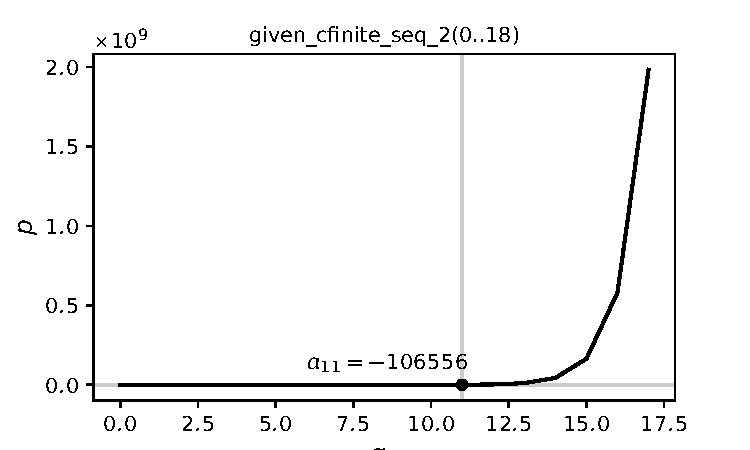
\includegraphics[width=1\linewidth]{../drawings/p5.pdf}
	%	\caption{}
	%	\label{fig:path1}
\end{figure}

\end{multicols}





\begin{lstlisting}

\end{lstlisting}








	





\section*{Source Code}
\href{https://github.com/AustinMaddison/discrete-simulation/tree/main/hw3/source}{https://github.com/AustinMaddison/discrete-simulation/tree/main/hw3/source}

% References
%\bibliographystyle{unsrt}
%\bibliography{references}

\end{document}
